\chapter{Implementation}\label{ch:impl}

As mentioned in \cref{sec:prep:goals}, the project involved two primary tasks executed concurrently.

The first was the extraction and description of the extensions to the Dataflow Model necessary for its implementation.
\Cref{sec:impl:dataflow} describes the results of this work in detail.

This extended model was then implemented in Elixir.
\Cref{sec:impl:approach} discusses several technical decisions made during this process.

\section{The Dataflow Model extended}\label{sec:impl:dataflow}

While the Dataflow paper \cite{Akidau:2015} summarised in \cref{sec:prep:dataflow} gives an overview of the Dataflow Model, it does not provide sufficient detail for its full implementation.
This section draws on many sources, including the Beam codebase \cite{Beam-code}, issue tracker \cite{Beam-JIRA}, and mailing list \cite{Beam-mailing} in order to compile the extensions to the Model necessary for a working implementation.

Many concepts in the Beam codebase are specific to the Java implementation.
Where the author felt this was the case, a more general concept was defined.
The need to implement these concepts in the very different Elixir language served as a good benchmark of which concepts were implementation details rather than necessary model changes.

This chapter does not aim to provide a full description of the Beam Model as it stands today.
Rather, it takes direction and inspiration from it to produce an extension to the Dataflow Model which enables Beam-like implementations of it to be built.

Finally, the project tackles only the data processing model itself.
Further extensions to the model are necessary---and present in Beam---to enable automated and efficient distribution of execution across a compute cluster.
These include checkpointing, serialisation and partitioning of data, and in themselves form a complex topic worthy of separate discussion.
Nevertheless, these concerns are outside the scope of this project and will only be mentioned tangentially where relevant.

\subsection{Pipelines, Transforms and Collections}\label{sec:impl:dataflow:pipelines-transforms-collections}

\emph{Pipelines} are independent namespaces of computation.
They are DAGs representing the flow of data through the system as it is transformed.

\begin{figure}[t]
	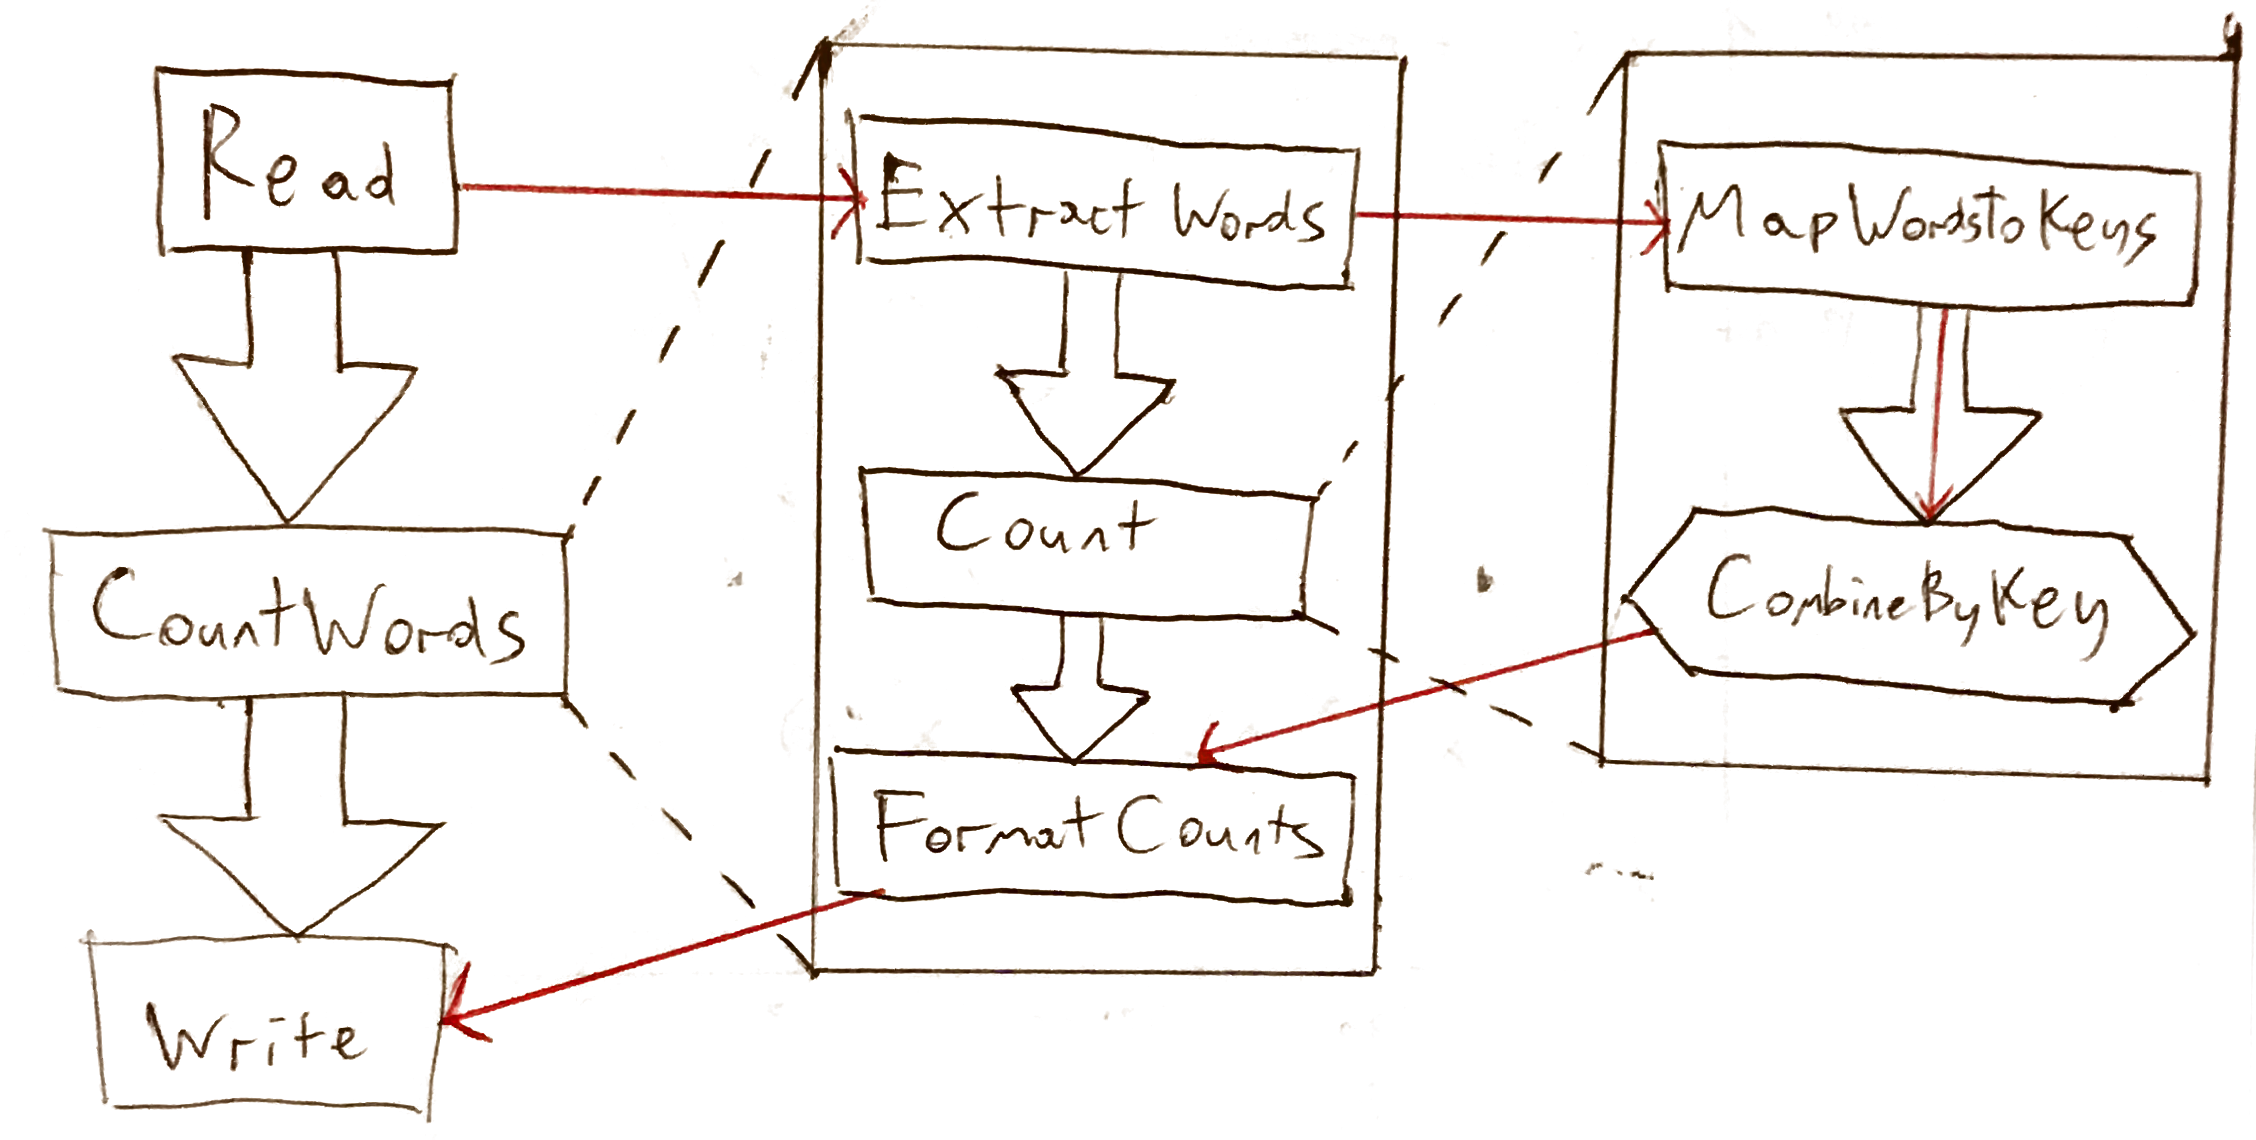
\includegraphics[width=\textwidth]{images/temp/composite-example}
	\caption[An illustration of the function of Composite Transforms in a typical Pipeline.]{A typical Pipeline uses Composite Transforms. The large arrows indicate the conceptual data flow path. The user expects to see visualisations or statistics using this abstraction. The thin red edges indicate the actual execution-time data flow---only leaf Transforms are instantiated and exchange data.}
	\label{fig:impl:composite-transforms}
\end{figure}

Each node in this graph is a \emph{Transform}.\footnote
{
In the Beam documentation and various other literature, these objects are called PTransforms and PCollections.
}
Transforms can have multiple inputs or outputs.

Each edge in the graph represents a \emph{Collection}.
It is a description of all the data that will ever be produced by a particular Transform.
Pipelines are constructed by \emph{applying} Transforms to Collections, resulting in a new Collection (or a structure grouping multiple new Collections).
This Collection encodes various information about the data, including the \emph{windowing strategy} the Collection will adopt and its producer.

We say that data is \emph{added} to a Collection whenever its producing Transform outputs data.
What this means in practice is implementation-dependent---Beam tracks Collections explicitly while the Elixir implementation uses them only to connect Transforms together, after which they exchange data directly.

Transforms may be Primitive or Composite---a Primitive Transform is directly executed by the Pipeline runner, while a Composite Transform \emph{expands} into multiple sub-Transforms at execution.
This is illustrated in \cref{fig:impl:composite-transforms}.
Different runners may choose to implement different Transforms as primitives and provide composite implementations for the rest.

Composite Transforms are tracked for informational purposes (statistics, logging or visualisation), but don't actually get instantiated at execution-time---they are merely a convenient abstraction for the user.

\subsubsection{Terminology}

There are three distinct types of entities which could reasonably be called Transforms.
The first is the class instance or structure which holds the parameters for the representation of the Transform and references its code at build-time.
We call this, as well as the relevant class or module itself, a \emph{Transform}.
This is what we actually apply to a Collection.

The result of such an application is a new Collection.
However, as a side effect, a node representing a particular instance of the Transform in a tree, with particular inputs and outputs, is added to the DAG.
We call such a node an \emph{Applied Transform}.
As well as the parameters of the Transform which was applied, it holds extra information which will be used at execution-time.

Finally, at execution-time, this Applied Transform will be instantiated into some runtime structure which is responsible for actually performing computation.
This may be an object in the case of Java or an actor process in the case of Elixir.
In any case we will call such an instance a \emph{Transform Executor}.

In sections where the intended meaning is clear, Transform may be used to refer to any of these.

\subsection{Windows and panes}\label{sec:impl:dataflow:windows-panes}

As described in \cref{sec:prep:dataflow:where}, \emph{windows} are used to group elements in event time (i.e.\ with regards to their intrinsic timestamps).
In practice, a window is merely a meta-value acting as a second key by which elements are grouped, usually taking the form of a time interval value.

What gives the Model its flexibility are \verb|WindowFn|s (windowing functions), described in \cref{sec:prep:dataflow:where}.
They are pairs of functions which can \emph{assign} windows to an element based on its timestamp and \emph{merge} multiple windows when needed.

We can draw a distinction between two classes of Transforms---\emph{Elementwise Transforms} and \emph{Grouping Transforms}.
They roughly correspond to the \verb|ParDo| / \verb|GroupByKey| distinction made in \cref{sec:prep:dataflow:what}.

Elementwise Transforms are essentially flat-map operations---they take input elements and for each one immediately output zero or more other elements.
It is possible for them to keep state, but most model pure functions.
Examples include \verb|Map|, \verb|FlatMap| and \verb|WindowInto|.

Grouping Transforms perform all operations partitioned by key and window.
They generally do not output any elements until they are triggered (as described below).
Much of the core complex logic of the Model deals with Grouping Transforms and ensuring they produce the correct data at the correct time.
Implementations make this behaviour available as a standard module or class to be used in such Transforms.

A \emph{pane} is an element produced by a Grouping Transform when a trigger fires, representing the output of that Transform for a given key and window.
It generally takes the form of a key-value pair.
For example, a \verb|GroupByKey| will output panes consisting of a key and a list of values which had that key and were in the given window.



\subsubsection{Watermark holds}

By default, each Transform Executor outputs a watermark which is equivalent to its input watermark, unless the output watermark is held back by a \emph{watermark hold}.
In that case, the output watermark is the earlier of the two.
Watermark holds provide a mechanism by which the Grouping Transform logic can hold back the output watermark until it is sure that it can satisfy the invariants described above.

Each Transform Executor has a \emph{watermark manager} which maintains a pair holds (the data hold and end-of-window/garbage-collection hold) per-window-per-key.
These are maintained separately so that they can be cleared and manipulated individually, but the overall watermark hold is simply their overall minimum.
Two holds are maintained for each window because some of the logic below requires us to know the data-derived hold even if the hold in effect is derived from the window only.

The data hold is, in effect, a reduction over all the element timestamps seen so far.
The exact reducing function is determined by the OutputTimeFn in use.
While the default simply sets all element timestamps to the end of their window---therefore making a reduction redundant as all inputs are always the same---other strategies are available such as `use the latest timestamp seen so far'.

\todo{diagrams diagrams diagrams}

The EOW/GC hold is a fallback used when we try to set a hold which cannot be honoured because either the output watermark has already progressed past it, or the input watermark has progressed beyond the EOW and therefore a timer to clear this hold won't be fired.
If we try to set an element hold in either of those situations, we automatically instead try to set the EOW/GC hold instead.

\todo{the below come out of specific invariants. Referencing them may make this shorter.}

An end-of-window hold is set in two situations:
\begin{itemize}
	\item The element is too late with respect to the output watermark to hold it back, but it may still be possible to include the element in an on-time pane.
	The EOW hold is placed to ensure that pane will not be considered late downstream.
	\item We must ensure that an on-time pane will be emitted for all windows which saw at least one element, even if that on-time pane is empty.
	Therefore, we place the EOW hold to ensure that this (possibly empty) pane will not be considered late downstream.
\end{itemize}

If the input watermark has progressed beyond the end-of-window, we can no longer place the EOW hold since a timer will not fire to clear it.
Instead, if the allowed lateness is non-zero, we try to set an additional garbage collection hold, which is analogous to the end-of-window hold but ensures that the panes we emit are at least non-droppable in the case they must be late.

When the trigger for a window fires, the hold for that window is cleared.
However, a garbage-collection hold may still remain for reasons described above.

It is important to keep in mind that when we talk about ``placing a hold'' below, we actually \emph{attempt} to place an element hold with a particular timestamp, at which point the above checks are performed and the appropriate hold set (or, possibly, no hold is set).
This allows for a decoupling of concerns in the two pieces of logic.


\subsection{Triggers and timers}\label{sec:impl:dataflow:triggers-timers}

In the previous section, we explored how Grouping Transforms accumulate data, ensure that their output watermark is held back until the aggregate is output, and mark their output appropriately to let the downstream know of the type of pane emitted.
However, it is still not clear how they know when they should produce some output at all.

The Model's answer to this is the trigger system.
Triggers were introduced in \cref{sec:prep:dataflow:when}, but this section aims to expand on their semantics and how they function to produce the desired behaviour.

\todo{should `trigger' be capitalised?}

\subsubsection{Triggers as state machines}
Once again, we draw the distinction between triggers at Pipeline-construction time, where they are simply bundles of configuration, and triggers (trigger drivers) at execution-time, where they do real work.
In this second case we can think of triggers as FSMs; indeed, the Beam implementation places its trigger logic in classes extending \verb|TriggerStateMachine|.

A trigger FSM is instantiated per-window-per-key and is used by the main Transform Executor to make decisions on when to output.
We say that a trigger \emph{fires} when it instructs the Transform Executor to output a pane.
Note that a trigger firing is binary---if it fires, all the currently accumulated data is output into a pane, which is timestamped and marked appropriately as detailed below.

We can easily see the overall behaviour of the FSM by looking at the \exs{TriggerDriver} behaviour from the Elixir implementation in \cref{lst:impl:trigger_driver}.

\begin{listing}[h]
	\begin{minted}{elixir}
defmodule Dataflow.DirectRunner.ReducingEvaluator.TriggerDriver do
  alias Dataflow.Utils.Time
  alias Dataflow.{Trigger, Window}
  
  @opaque state :: any
  @callback init(Trigger.t, Window.t, timing_manager :: pid) :: state
  @callback process_element(state, Time.timestamp) :: state
  @callback merge([state], state) :: state
  @callback should_fire?(state) :: boolean
  @callback fired(state) :: state
  @callback finished?(state) :: boolean
end
	\end{minted}
\caption[The \exs{TriggerDriver} behaviour showing the Finite State Machine design of an execution-time trigger.]{The \exs{TriggerDriver} behaviour showing the FSM design of an execution-time trigger. The \exs{timing_manager} passed to the \exs{init} function is the \exs{pid} of the current Transform's timing manager, allowing the trigger driver to set and clear timers and access current watermark state.}
\label{lst:impl:trigger_driver}
\end{listing}

\todo{Consider using the Elixir type syntax everywhere in this chapter to specify the different structures being talked about (instead of prose)}

There we see that the FSM is first initialised (\exs{init}) with trigger and window data (along with a handle to a process which allows it to set and clear timers asynchronously, as well as read the watermarks and processing time).
It then receives a series of \exs{process_element} calls, receiving the timestamps of elements being processed and being allowed to update its state.
It will optionally be asked to \exs{merge} its state with that of other windows---typically we require that the actual trigger being used is the same in all cases.

Note that the trigger driver itself does not asynchronously notify the transform executor of its firing.
Instead, the transform executor will ask the trigger driver if it is ready to fire using \exs{should_fire?}.
If so, a pane of output is produced and the trigger driver is notified via the \exs{fired} callback.

A trigger is \emph{closed} or \emph{finished} if it will never fire again.
The trigger driver can be asked if it is finished using the \exs{finished?/1} callback.
At that point it is safe to garbage-collect the associated window state, leaving only a tombstone indicating that new elements placed in this window should be ignored.
Once the $\mathit{LIWM}$ passes the GC time of the window, we can delete this tombstone as well.

It is clear that this model allows great flexibility in specifying exactly when output should occur.
The FSM can count elements, set timers for particular event or processing times, and flexibly decide if it will fire multiple times.
The model could also be extended to support punctuations (data-driven triggers) by allowing \exs{process_element} to inspect the element value itself.
This is not implemented, but being worked on, in Beam <JIRA ref> and was considered out-of-scope for the Elixir implementation.

It should be noted that a standard pattern in the Model is to use composite triggers---for example, a trigger which fires when trigger A \emph{or} trigger B fire, or one which takes a one-time firing trigger A (one which becomes finished after firing once) and instead resets it after each firing, making it able to fire indefinitely.
This is enabled by the decoupled design of trigger drivers, allowing them to be queried by a parent trigger just as easily as they could be queried by the transform executor itself, resulting in a tree of triggers.

\subsubsection{Example: The default trigger}

The \emph{default trigger} used when no other trigger is explicitly specified fires once when the event watermark passes the end-of-window, and fires again every single time a late element is seen (producing a one-element late pane with that element).

\Cref{lst:impl:default_trigger} illustrates the simple logic needed to accomplish this behaviour.
\todo{insert listing here, without private helper functions.}

\subsubsection{Timers}

Timers are a simple but flexible way to schedule asynchronous action in the future.
A \emph{timer} is a tuple of \exs{{namespace, time, domain}}\footnotemark, with the \exs{domain} being one of processing-time or event-time.
A \emph{timing manager} is instantiated per Transform Executor, though it operates asynchronously to the Transform Executor itself.
It handles watermark management and timers.

\footnotetext
{
In Beam, timers also have a unique ID, in order to identify and compare their identity. This is not needed in Elixir, since they can be directly compared value-wise.
}

Once a timer is set, the timing manager will notify the Transform Executor once it fires.
This will happen when the input watermark (event time) or clock time (processing time) \textbf{passes} the time of the timer; that is, when the appropriate time measure is \textbf{strictly greater} than the time of the timer.
A maximal event-time timer fires precisely when that time is reached, since time cannot advance past it.
Multiple timers may fire simultaneously, and the Transform Executor will be notified of all of them.

The \exs{namespace} of a timer is an arbitrary value, but in practice is used to associate timers to the triggers that set them, or to keep track of different timer purposes in custom implementations.
Often (e.g.\ in the Grouping Transform) the namespace is not even read on a timer firing (all timers are treated the same), but rather only employed to clear specific timers before they fire.

It is important to note that no semantics are implied by the timers themselves---they merely provide a mechanism to receive a notification with a particular identifier at a particular time.
It is up to the Transform Executor to interpret this and act accordingly.

In the case of a Grouping Transform, on receiving a timer the Executor asks the trigger driver whether it should fire.
The trigger has access to the current watermark state, and so can determine whether it is time to fire.
The flexible implementation means that it another timer could be set at this point, enabling strategies such as `output a pane every five seconds until the end of the window, but only if we've seen 10 elements or more'.

\subsection{Watermark generation and processing}\label{sec:impl:dataflow:watermark-generation}

\todo{diagram}

In \cref{sec:impl:dataflow:lateness} it was asserted that only late input can result in late data anywhere in the system.
Late input was also defined as that whose timestamp falls behind the current input watermark.
The previous sections also detail the exact semantics necessary to preserve watermark correctness along with many useful invariants throughout the whole Pipeline.

However, none of the preceding sections address the question of generating a watermark in the first place.
This process is crucial---as mentioned above, it is the only part of the system in which lateness can be introduced.

It also very application-specific.
A watermark is an indication of the progress made so far in the event stream.
For some data sources, we can get a guaranteed-correct read-position.
For others, the source provides us with only an approximation.
In yet other cases, we must keep statistics about the source to generate a heuristic ourselves.

Clearly there is no standard solution---there must be a mechanism to allow flexibility in watermark generation.
We introduce the standard concept of a \emph{Source}, which can produce a Collection from some external source when coupled with a \verb|Read| Transform.

At execution, the \verb|Read| Transform Executor will use logic found in the Source it is given in order to assign timestamps to elements being read (usually an intrinsic timestamp in the case of e.g.\ Kafka messages) and to publish a monotonically increasing watermark.
Bounded sources with no intrinsic timestamps will generally output a minimal watermark (and timestamp all output with the minimal timestamp) until it is finished, advancing the watermark to the maximal timestamp to indicate that.

Sources for popular data sources such as the file system, Apache Kafka, Google BigQuery and others are included in the Beam implementation, and an API is provided to add custom ones with arbitrary watermark logic (in fact, this API is used in \cref{sec:eval:code}).

\subsubsection{Watermark domains}

Forcing the Source to generate the original input watermark works well from a system perspective, providing a single, easily-managed point where lateness can be introduced.
However, it can cause problems from a user perspective and limit the flexibility of the Model.

Suppose a Pipeline is receiving data containing names of log files in cloud storage.
These files contain log entries collected during a particular day, which are then dumped to storage during log rotation every 24 hours.
The timestamp of these elements will be the timestamp of the file, which will be \textbf{after} all of the entries in the file.

This means that if we were to process the file contents in a Transform and output all the log entries within as individual elements, all those elements would have to be output late if they kept their real timestamps.
They could avoid being dropped by selecting an appropriate value for the allowed lateness, but that is a misuse of the Model and semantically incorrect.

In fact, these new elements are not late, because they belong in a different \emph{watermark domain} than the files containing them.
Collections can be thought of as being in the same watermark domain when their elements' timestamps directly relate to one another \textbf{independently of the element data}.
For example, when extracting body text from a social post, it makes sense to assign the same timestamp to the text as was assigned to the post itself.
We don't need to actually look at the post to make that decision.
Similarly, a Grouping Transform treats data aggregation and timestamp aggregation orthogonally.

\todo{diagram}

However, in the log-file example given, the timestamp of an individual log entry generated from a file will be dependent on the data of the log entry itself---the recorded time of its generation.
We may be able to provide a guarantee such as `the timestamp of an entry will never be earlier than 24 hours before the timestamp of a file', but this again is an application-specific decision, unsuitable for inclusion in a generic model.

Such a guarantee also constitutes precisely what a watermark is.
Alas, in order to have a predictable lateness model, we have constrained the output watermark of a Transform to always be less than or equal to its input watermark.
Shifting our watermark to 24 hours before the input watermark would violate this invariant.

The solution is to break our Pipeline into several watermark domains.
The invariants and relationships described in this chapter hold only within one watermark domain---we are essentially treating each one of these as a mini-Pipeline of its own.

Similarly to how event-time and processing-time are distinguished, we now treat event-time as a \emph{class} of domains rather than a single domain of its own.

The lateness semantics only make sense when applied to data which can all be semantically described with one time domain.
Once we switch semantic time domains, there is no general solution to obtaining the correct watermark---the problem once-again becomes application-specific.
This is the same problem faced when considering the initial input data into the Pipeline, and so it makes sense for it to be solved similarly.

We introduce a type of Transform which initiates a new watermark domain.
These Transforms may directly manage their own output watermark, which does not need to (but can) have a formulaic relation to their input watermark.

This, of course, introduces a potential source of lateness at every point such a Transform is placed in the Pipeline.
However this too semantically makes sense.
At these points, we are essentially reading a conceptually new, external Collection of elements, with timing information which did not exist in the Pipeline until this point.
Since this information is unavailable before this point, it is impossible for the previous transformations to have taken account of it in determining whether input to the system was late.

The watermark domain solution is the proposal of the author and is not in place in the Beam Model.
It is included in the Elixir implementation of the Model.
There is no accepted general solution to this problem in the Beam community.

The proposed solution also potentially simplifies the original approach to Sources.
An example of this can be seen in one of the Evaluation examples (\cref{sec:todo}).


\section{The Dataflow Model implemented}\label{sec:impl:approach}

\subsection{The Dataflow DSL}\label{sec:impl:approach:dsl}

An important component of this project, and one of its original goals, was the design of a readable, approachable DSL for constructing pipelines.

As described in \cref{sec:prep:elixir:basics}, Elixir has a commonly-used pipeline operator \exs{|>}, and programmers are encouraged to express their programs using series of data transformations.
Thus, the Dataflow way of expressing computation translates quite naturally into Elixir, and only a minimal amount of additional syntax is necessary.

\begin{listing}[h]
	\caption[An example of Pipeline construction in Elixir.]{An example of Pipeline construction in Elixir. A Pipeline is created, and to it are applied Transforms which count the words in a file and output these counts to a new file. The Pipeline is then executed.}
	\label{lst:impl:elixir-construct-pipeline}
	\begin{minted}{elixir}
use Dataflow
alias Dataflow.Transforms.{Core, IO, Aggregation}
alias Dataflow.DirectRunner

pipeline = Pipeline.new

pipeline
~> IO.read_file("data/data1.txt")
~> Aggregation.count_elements()
~> "Format Counts" -- Core.map(fn {word, count} -> "#{word}: #{count}" end)
~> IO.write_file("data/output.txt")

DirectRunner.run pipeline, sync: true

	\end{minted}
\end{listing}

\Cref{lst:impl:elixir-construct-pipeline} illustrates the API with a very simple, but working example.
We read a file which contains a single word on each of its lines.
We count the number of occurrences of each word, format this information and output it to another file.

The code is clear and understandable, and maps very well to the Elixir model of data processing.
\Cref{fig:todo} shows this Pipeline as a DAG.

\todo{diagram of pipeline}

In line 10, we see the \exs{--} operator being used to assign a label to a particular Transform.
Assigning labels to transforms is an important feature, very useful for managing and visualising Pipelines.
This notation evokes the use of \verb|--| to denote a dash in \LaTeX.

\begin{listing}[h]
	\caption{An implementation of the process in \cref{lst:impl:elixir-construct-pipeline} using regular, sequential functions.}
	\label{lst:impl:elixir-normal-comparison}
	\begin{minted}{elixir}
input = File.stream!("data/data1.txt")
output = File.stream!("data/output.txt", [:write])

input
|> count_elements() # helper function
|> Enum.map(fn {word, count} -> "#{word}: #{count}" end)
|> Enum.into(output)
	\end{minted}
\end{listing}

\Cref{lst:impl:elixir-normal-comparison} shows, for comparison, how this process would usually be implemented using normal, sequential processing in Elixir.
The most obvious difference between this listing and \cref{lst:impl:elixir-normal-comparison} is that in the latter, we include an extra \exs{pipeline} identifier which has to explicitly be \exs{run}.
This makes sense, as the Model requires us to separate the description of the computation in the construction phase from its execution in the subsequent phase.

\subsubsection{Using macros}

Those with a passing familiarity with Elixir will recognise that \exs{--} is actually the list difference operator.
While it would be possible to have the \exs{use Dataflow} statement replace the default \exs{--} with a version used for labelling Transforms, it would likely cause confusion.
How then is this entire syntax implemented?

The answer is that \exs{~>} is in fact a macro.
Elixir macros are powerful tools, allowing arbitrary AST transformation at compile time <ref to bbook>.
They can also cause unexpected behaviour and confusion, and the convention is to keep their use minimal, relying on functions instead.
This is why the definition of \exs{~>} is only a few lines long, shown in \cref{lst:impl:elixir-dpipe-macro-def}.

\begin{listing}[h]
	\caption{The definition of the \exs{~>} macro, showcasing the usefulness and power of Elixir macros.}
	\label{lst:impl:elixir-dpipe-macro-def}
	\begin{minted}[autogobble]{elixir}
 defmacro pvalue ~> transform_with_label do
    case transform_with_label do
      {:--, _, [label, transform]} ->
        quote bind_quoted: [pvalue: pvalue, transform: transform, label: label] do
          Dataflow.__apply_transform__(pvalue, transform, label)
        end
      transform ->
        quote bind_quoted: [pvalue: pvalue, transform: transform] do
          Dataflow.__apply_transform__(pvalue, transform)
        end
    end
  end
	\end{minted}
\end{listing}

Macros are simply functions which, at compile-time, take the Abstract Syntax Trees (ASTs) of their arguments and output an AST with which they are replaced.

The \exs{~>} macro works by pattern-matching on the structure of the second argument, which will either be an AST node of the form \exs{label -- transform} (line 3) or something else (line 7).
The macro outputs a new AST node which simply calls the \exs{Dataflow.__apply_transform__} function which contains the Transform application logic.
This matching at the AST level means that we are free to assign \exs{--} a new definition only within this expression, without needing to shadow the original meaning for the entire namespace.

We do not have to manually construct the replacement AST node---the \exs{quote} macro allows us to create one by simply writing syntax and specifying which variables from the macro's environment we want to bind to the environment of the resultant AST node (the \exs{:bind_quoted} option).

The only other piece of magic present is the \exs{use Dataflow} line, which imports the \exs{~>} macro so that it can be used straight away.
In fact, that line of code simply calls the \exs{Dataflow.__using__} macro.
In this way, Elixir allows developers to strike a good balance between friendliness and ease-of-use, and explicitness, which is very desirable when things go wrong.

Intuitively, the result of an application of the \exs{~>} operator is a \emph{Value}, which is either a Collection or some compound (e.g.\ a tuple) containing Collections.
We can hold on to Collections that are returned in this way and apply Transforms to them several times.
This means that we can create branching Pipelines such as the one in \cref{fig:todo} easily, as shown in \cref{lst:impl:diverging-pipelines}.

In order to instantiate a Root Transform (one which produces data obtained outside the system somehow), we apply it to the Pipeline itself.

\begin{listing}[h]
	\caption{Branching Pipelines can be created by applying multiple Transforms to the same Collection.}
	\label{lst:impl:diverging-pipelines}
	\begin{minted}[autogobble]{elixir}
pipeline = Pipeline.new

words =
  pipeline
  ~> IO.read_file("data.txt")
  ~> extract_words()
  
# save words to file
words ~> IO.write_file("words.txt")

# also get the top words and write them to another file
words
~> get_top_words()
~> IO.write_file("top_words.txt")
	\end{minted}
\end{listing}

\subsubsection{Structs and protocols}

Since there is a need to separate the construction and execution phases of the Model, the situation cannot be as simple as in \cref{lst:impl:elixir-normal-comparison}, where on passing a value to a `transformation', we simply call the function directly.
Instead, we must store the description of the computation in the Pipeline structure.

In order to facilitate this, we make use of Elixir's protocols and structs.
A struct is a map with a special \exs{:__struct__} key, which exhibits some special behaviour at compile-time.
A struct is always associated with a particular module.

A protocol is an interface module consisting of a set of function declarations.
Implementations of a protocol can then be defined on a per-module basis, as long as that module declares a struct.
When the protocol functions are then called with a struct whose module implements that protocol, the actual function called will be dynamically dispatched to that module.

The functions in \cref{lst:impl:elixir-construct-pipeline}, such as \exs{IO.read_file}, don't perform any computation themselves---instead, they return a struct which stores the arguments passed in and implements the \exs{PTransform.Callable} protocol.
For example, the result of calling \linebreak \exs{IO.read_file("data.txt")} is \mintinline{elixir}{
%IO.ReadFile{filename: "data.txt"}
}.

The definition of \exs{~>} in \cref{lst:impl:elixir-dpipe-macro-def} shows that these structs are subsequently incorporated into the Pipeline by calling the appropriate function which internally uses the protocol.

The definition of the Transform protocol is presented in \cref{lst:impl:ptransform-callable}.
We see that the only requirement is for the Transform to be able to expand to more Transforms, following the Composite Transforms concept introduced earlier.
Primitive Transforms are not definable by the user and receive special treatment, but the user is free to define their own Composite Transforms by providing an appropriate structure and module, much like one would define small, composable functions.
It is technically possible to use a function which composes Transforms internally, but this means that this new Transform is not recognised as a node, leading to a poorer experience once visualisation and/or reporting is introduced.

\todo{insert PTransform protocol}

\subsubsection{Managing DAGs using asynchronous processes}

\todo{ref to a paper on implementing functional dags in Haskell?}

Constructing and working with DAGs in the absence of mutability, especially when advanced functional features such as those found in e.g.\ Haskell are not available, lies somewhere between impossible and infeasible.
Instead of attempting to do this, the concurrency model of Elixir was leveraged to simulate a mutable map of Collections and Applied Transforms inside the Pipeline structure.

\todo{mention that Erlang's :digraph library also uses mutable state but is unsuitable for use here?}

The call to \exs{Pipeline.new} actually starts a new process which contains a map of the Collections (edges) and Applied Transforms (nodes) in the Pipeline graph, indexed by a unique integer ID.
This means that it is possible to easily add new structures to the DAG, even in the face of Composite Transforms or branching Pipelines.

It is clear from \cref{lst:impl:diverging-pipelines} that Pipelines behave like mutable objects---merely using the \exs{~>} operator on a Pipeline modifies it.
Therefore Pipelines in this state are better thought of as processes rather than values.
However, once the construction of the Pipeline is finished, it is possible to freeze it and turn it into a simple data structure which once again behaves in the expected manner.
Indeed, the \exs{DirectRunner.run} function does this internally before taking this data structure and executing it.

\subsection{Making state explicit}\label{sec:impl:approach:state-explicit}

\todo{discuss moving from a stateful approach where things can just grab state out of thin air and mutate it, into an explicit approach of functions taking state and returning a modified version of the state. Also expand on how this forces greater focus on what a particular function actually does as it needs to explicitly receive things it needs, and explicitly return things it touches/modifies.}

\subsection{Managing concurrency with OTP and GenServers}\label{sec:impl:approach:concurrency}

\todo{Introduce the concept of OTP, GenServers and how they provide robust, serialised concurrency. Make clear how building on top of these core libraries is advantageous and appropriate. Mention how clear semantics enable concurrency design.}

\subsection{The GenStage library}\label{sec:impl:approach:genstage}

\todo{Introduce concept of GenStage and how it builds on GenServer. Mention how its operation is a great fit for the type of computation being done in Dataflow.}

\subsection{Extensibility using behaviours and protocols}\label{sec:impl:approach:extensibility}
